% CS669: Pattern Recognition
% Programming Assignment II
% Gabriel Dulac-Arnold <gabe@squirrelsoup.net>
% Johannes H. Jensen <johannj@stud.ntnu.no>
\documentclass[a4paper]{article}
\usepackage{multicol}
\usepackage{graphicx}
\usepackage[top=2cm,nohead,nofoot]{geometry}

\author{Gabriel Dulac-Arnold $<$gabe@squirrelsoup.net$>$ (CS09F004) \\
Johannes H. Jensen $<$johannj@stud.ntnu.no$>$ (CS09F005) \\
\\
(Batch no. 14)}
\title{CS669 - Pattern Recognition\\
\emph{Programming Assignment II}}

\begin{document}
\setlength{\parskip}{2ex}
\setlength{\tabcolsep}{8pt}
\renewcommand\arraystretch{1.5}
\maketitle

\section{Dataset I: Nonlinearly Separable}

Expectation Maximization was run for estimating the parameters of the
classifier based on Gaussian Mixture Models with increasing values of $K$.
For $K=11$ the classifier achieved 100\% accuracy on the training data:

\begin{verbatim}
Trying K=1... Evaluating... 62.61% accuracy
Trying K=2... Evaluating... 73.24% accuracy
Trying K=3... Evaluating... 75.03% accuracy
Trying K=4... Evaluating... 84.63% accuracy
Trying K=5... Evaluating... 92.40% accuracy
Trying K=6... Evaluating... 92.51% accuracy
Trying K=7... Evaluating... 98.17% accuracy
Trying K=8... Evaluating... 99.18% accuracy
Trying K=9... Evaluating... 99.26% accuracy
Trying K=10... Evaluating... 99.89% accuracy
Trying K=11... Evaluating... 100.00% accuracy
\end{verbatim}

The $h$ values for the hyperpshere Parzen method was chosen by iterating 
values of $h$ with until the best performance was achieved.  Due to the 
high value of $h$ for the real world data set, a step size of 100 was chosen. 
The value for $h$ was only empirically chosen using the hypersphere method. 

Our implementation of the gaussian method is not terribly fast, so we simply
re-used the values of $h$ that worked well with the hypersphere method for 
the gaussian method. After a bit of manual verification, this assumption 
seems to be acceptable.

Selection of k for Bayesian KNN was done iteratively until accuracy was 
maximal and stable.

\subsection{Classifier Accuracy}

\begin{tabular}{ | l | r | }
\hline
\textbf{Classifier} & \textbf{Accuracy} \\
\hline
Bayes $GMM_{11}$, Diagonal covariance matrix  &   98.94\% \\
Bayes $GMM_{11}$, Full covariance matrix      &   100\%   \\
\hline
Bayes $Parzen_{15}$, Hypersphere as region    &   100\%   \\
Bayes $Parzen_{15}$, Gaussian kernel          &   97.06\% \\
\hline
Bayes $KNN_15$                                &   100\%   \\
\hline
KNN, $K=1$                                    &   100\%   \\
KNN, $K=20$                                   &   100\%   \\
KNN, $K=40$                                   &   100\%   \\
KNN, $K=60$                                   &   100\%   \\
\hline
\end{tabular}


\subsection{Confusion Matrices}

\begin{multicols}{2}
\begin{enumerate}
\item Bayes $GMM_{11}$, Diagonal cov matrix:

\begin{tabular}{ | l | c | c | }
\hline
& $\omega_1$ & $\omega_2$ \\
\hline
  $\omega_1$ & 606 & 6 \\
\hline
  $\omega_2$ & 7 & 605 \\
\hline
\end{tabular}


\item Bayes $GMM_{11}$, Full covariance matrix:

\begin{tabular}{ | l | c | c | }
\hline
& $\omega_1$ & $\omega_2$ \\
\hline
  $\omega_1$ & 612 & 0 \\
\hline
  $\omega_2$ & 0 & 612 \\
\hline
\end{tabular}


\item Bayes $Parzen_{15}$, Hypersphere as region

\begin{tabular}{ | l | c | c | }
\hline
& $\omega_1$ & $\omega_2$ \\
\hline
  $\omega_1$ & 612 & 0 \\
\hline
  $\omega_2$ & 0 & 612 \\
\hline
\end{tabular}



\item Bayes $Parzen_{15}$, Gaussian kernel

\begin{tabular}{ | l | c | c | }
\hline
& $\omega_1$ & $\omega_2$ \\
\hline
  $\omega_1$ & 593 & 19 \\
\hline
  $\omega_2$ & 17 & 595 \\
\hline
\end{tabular}


\item Bayes $KNN_{15}$

\begin{tabular}{ | l | c | c | }
\hline
& $\omega_1$ & $\omega_2$ \\
\hline
  $\omega_1$ & 612 & 0 \\
\hline
  $\omega_2$ & 0 & 612 \\
\hline
\end{tabular}


\item $KNN$, $K \in \{1,20,40,60\}$

\begin{tabular}{ | l | c | c | }
\hline
& $\omega_1$ & $\omega_2$ \\
\hline
  $\omega_1$ & 612 & 0 \\
\hline
  $\omega_2$ & 0 & 612 \\
\hline
\end{tabular}

\end{enumerate}
\end{multicols}


\newpage
\subsection{Decision Region Plots}

\begin{figure}[htbp!]
\center
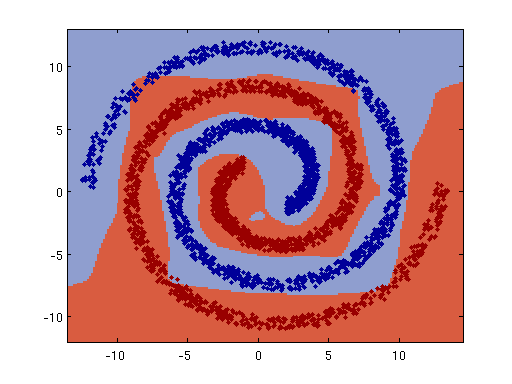
\includegraphics[clip, trim=40px 15px 30px 10px]{gmm_nls_diagcov.png}
\caption{Bayes $GMM_{11}$, Diagonal covariance matrix}
\end{figure}

\begin{figure}[htbp!]
\center
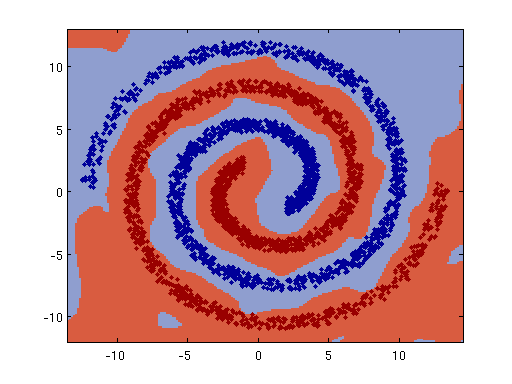
\includegraphics[clip, trim=40px 15px 30px 10px]{gmm_nls_fullcov.png}
\caption{Bayes $GMM_{11}$, Full covariance matrix}
\end{figure}

\begin{figure}[htbp!]
\center
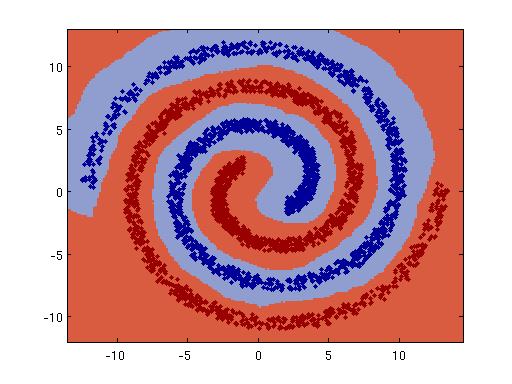
\includegraphics[clip, trim=40px 15px 30px 10px]{parzen_nls_sphere.png}
\caption{Bayes $Parzen_{15}$, Hypersphere as region}
\end{figure}

\begin{figure}[htbp!]
\center
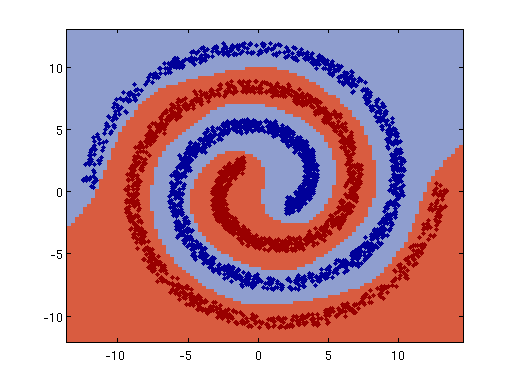
\includegraphics[clip, trim=40px 15px 30px 10px]{parzen_nls_gauss.png}
\caption{Bayes $Parzen_{15}$, Gaussian kernel}
\end{figure}

\begin{figure}[htbp!]
\center
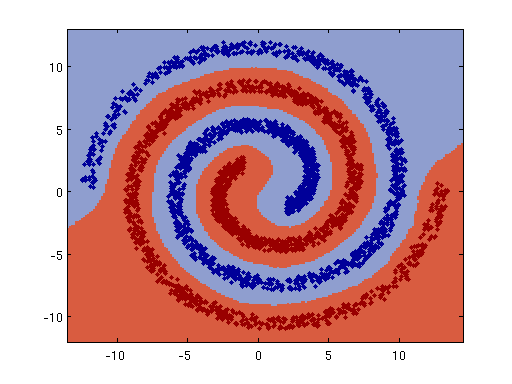
\includegraphics[clip, trim=40px 15px 30px 10px]{bayes_knn_nls.png}
\caption{Bayes $KNN_{15}$}
\end{figure}

\begin{figure}[htbp!]
\center
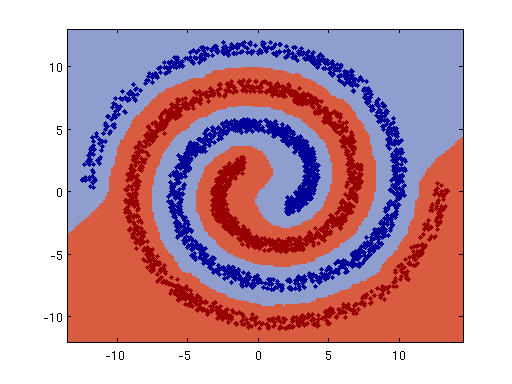
\includegraphics[clip, trim=40px 15px 30px 10px]{knn_nls.png}
\caption{KNN, $K \in \{1,20,40,60\}$}
\end{figure}






\newpage
\section{Dataset II: Real World Dataset}

Expectation Maximization was run for estimating the parameters of the
classifier based on Gaussian Mixture Models with increasing values of $K$.
The values of K did not seem to give an apparent increase in accuracy:

\begin{verbatim}
Trying K=1... Evaluating... 96.49% accuracy
Trying K=2... Evaluating... 98.10% accuracy
Trying K=3... Evaluating... 97.91% accuracy
Trying K=4... Evaluating... 97.91% accuracy
Trying K=5... Evaluating... 98.11% accuracy
\end{verbatim}

Since the real world dataset contains overlapping data, an accuracy of 100\%
is only achievable when K approaches the number of data points. Thus we settled
for K=2.


\subsection{Classifier Accuracy}

\begin{tabular}{ | l | r | }
\hline
\textbf{Classifier} & \textbf{Accuracy} \\
\hline
Bayes $GMM_{2}$, Diagonal covariance matrix   &   88.57\% \\
Bayes $GMM_{2}$, Full covariance matrix       &   88.29\% \\
\hline
Bayes $Parzen_{1500}$, Hypersphere as region  &   85.99\% \\
Bayes $Parzen_{1500}$, Gaussian kernel        &   88.29\% \\
\hline
Bayes $KNN_{15}$                              &   87.21\% \\
\hline
KNN, $K=1$                                    &   84.70\% \\
KNN, $K=20$                                   &   86.98\% \\
KNN, $K=40$                                   &   87.03\% \\
KNN, $K=60$                                   &   86.86\% \\
\hline
\end{tabular}


\newpage
\subsection{Confusion Matrices}

\begin{multicols}{2}
\begin{enumerate}
\item Bayes $GMM_{2}$, Diagonal cov matrix:

\begin{tabular}{ | l | c | c | c | }
\hline
& $\omega_1$ & $\omega_2$ & $\omega_3$ \\
\hline
  $\omega_1$ & 587 & 7 & 3 \\
\hline
  $\omega_2$ & 169 & 388 & 16 \\
\hline
  $\omega_3$ & 2 & 0 & 620 \\
\hline
\end{tabular}


\item Bayes $GMM_{2}$, Full covariance matrix:

\begin{tabular}{ | l | c | c | c | }
\hline
& $\omega_1$ & $\omega_2$ & $\omega_3$ \\
\hline
  $\omega_1$ & 587 & 7 & 3 \\
\hline
  $\omega_2$ & 173 & 385 & 15 \\
\hline
  $\omega_3$ & 4 & 0 & 618 \\
\hline
\end{tabular}


\item Bayes $Parzen_{1500}$, Hypersphere as region

\begin{tabular}{ | l | c | c | c | }
\hline
& $\omega_1$ & $\omega_2$ & $\omega_3$ \\
\hline
  $\omega_1$ & 588 & 6 & 3 \\
\hline
  $\omega_2$ & 199 & 361 & 13 \\
\hline
  $\omega_3$ & 18 & 4 & 600 \\
\hline
\end{tabular}


\item Bayes $Parzen_{1500}$, Gaussian kernel

\begin{tabular}{ | l | c | c | c | }
\hline
& $\omega_1$ & $\omega_2$ & $\omega_3$ \\
\hline
  $\omega_1$ & 579 & 15 & 3 \\
\hline
  $\omega_2$ & 352 & 206 & 15 \\
\hline
  $\omega_3$ & 0 & 0 & 622 \\
\hline
\end{tabular}

\columnbreak

\item Bayes $KNN_{15}$

\begin{tabular}{ | l | c | c | c | }
\hline
& $\omega_1$ & $\omega_2$ & $\omega_3$ \\
\hline
  $\omega_1$ & 568 & 26 & 3 \\
\hline
  $\omega_2$ & 174 & 381 & 18 \\
\hline
  $\omega_3$ & 0 & 0 & 622 \\
\hline
\end{tabular}


\item $KNN_{1}$

\begin{tabular}{ | l | c | c | c | }
\hline
& $\omega_1$ & $\omega_2$ & $\omega_3$ \\
\hline
  $\omega_1$ & 571 & 23 & 3 \\
\hline
  $\omega_2$ & 224 & 335 & 14 \\
\hline
  $\omega_3$ & 0 & 0 & 622 \\
\hline
\end{tabular}


\item $KNN_{20}$

\begin{tabular}{ | l | c | c | c | }
\hline
& $\omega_1$ & $\omega_2$ & $\omega_3$ \\
\hline
  $\omega_1$ & 567 & 27 & 3 \\
\hline
  $\omega_2$ & 177 & 378 & 18 \\
\hline
  $\omega_3$ & 0 & 0 & 622 \\
\hline
\end{tabular}


\item $KNN_{40}$

\begin{tabular}{ | l | c | c | c | }
\hline
& $\omega_1$ & $\omega_2$ & $\omega_3$ \\
\hline
  $\omega_1$ & 569 & 25 & 3 \\
\hline
  $\omega_2$ & 178 & 377 & 18 \\
\hline
  $\omega_3$ & 0 & 0 & 622 \\
\hline
\end{tabular}


\item $KNN_{60}$

\begin{tabular}{ | l | c | c | c | }
\hline
& $\omega_1$ & $\omega_2$ & $\omega_3$ \\
\hline
  $\omega_1$ & 568 & 26 & 3 \\
\hline
  $\omega_2$ & 179 & 375 & 19 \\
\hline
  $\omega_3$ & 0 & 0 & 622 \\
\hline
\end{tabular}

\end{enumerate}
\end{multicols}


\newpage
\subsection{Decision Region Plots}

\begin{figure}[htbp!]
\center
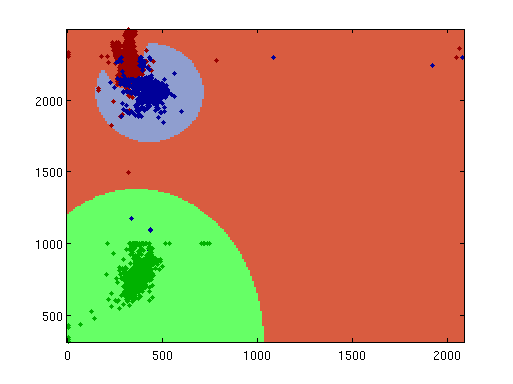
\includegraphics[clip, trim=40px 15px 30px 10px]{gmm_real_diagcov.png}
\caption{Bayes $GMM_{2}$, Diagonal covariance matrix}
\end{figure}

\begin{figure}[htbp!]
\center
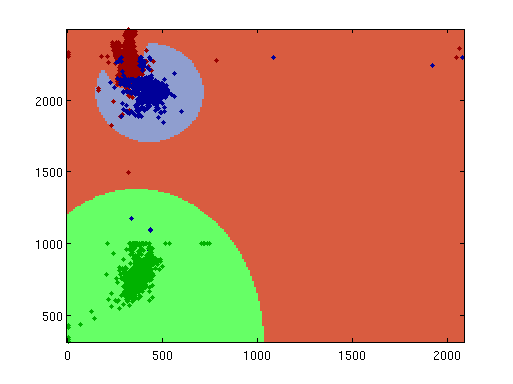
\includegraphics[clip, trim=40px 15px 30px 10px]{gmm_real_fullcov.png}
\caption{Bayes $GMM_{2}$, Full covariance matrix}
\end{figure}

\begin{figure}[htbp!]
\center
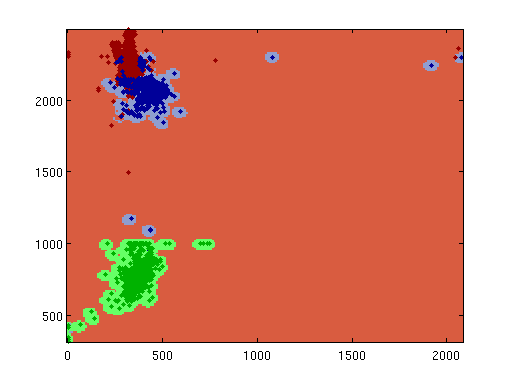
\includegraphics[clip, trim=40px 15px 30px 10px]{parzen_real_sphere.png}
\caption{Bayes $Parzen_{1500}$, Hypersphere as region}
\end{figure}

\begin{figure}[htbp!]
\center
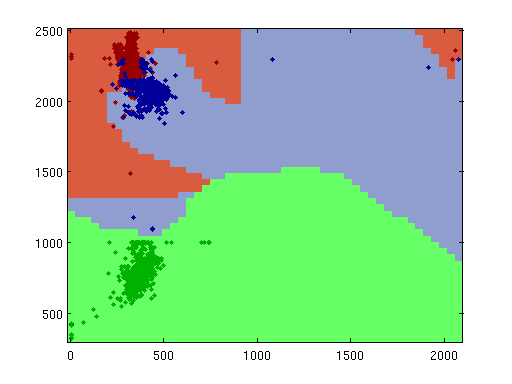
\includegraphics[clip, trim=40px 15px 30px 10px]{parzen_real_gauss.png}
\caption{Bayes $Parzen_{1500}$, Gaussian kernel}
\end{figure}

\begin{figure}[htbp!]
\center
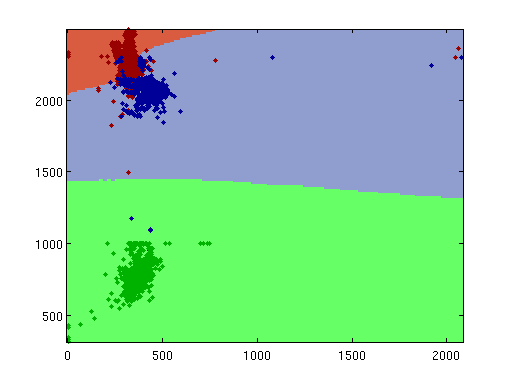
\includegraphics[clip, trim=40px 15px 30px 10px]{bayes_knn_real.png}
\caption{Bayes $KNN_{15}$}
\end{figure}

\begin{figure}[htbp!]
\center
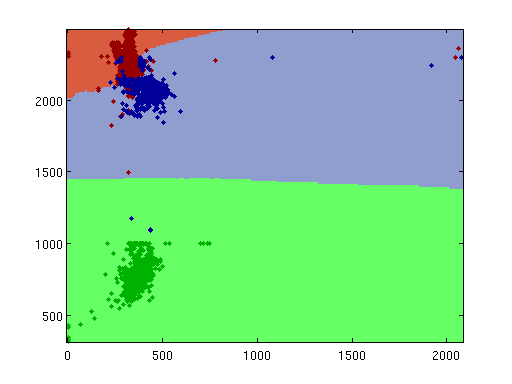
\includegraphics[clip, trim=40px 15px 30px 10px]{knn_real.png}
\caption{KNN, $K=1$}
\end{figure}

\begin{figure}[htbp!]
\center
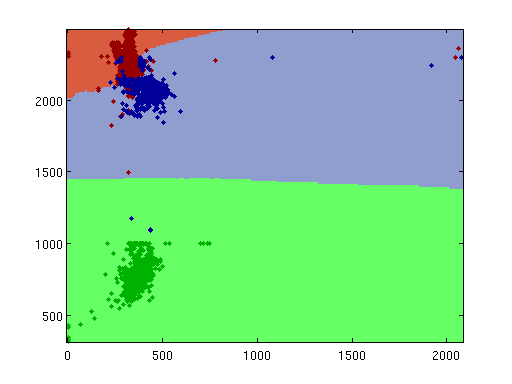
\includegraphics[clip, trim=40px 15px 30px 10px]{knn_real.png}
\caption{KNN, $K=20$}
\end{figure}

\begin{figure}[htbp!]
\center
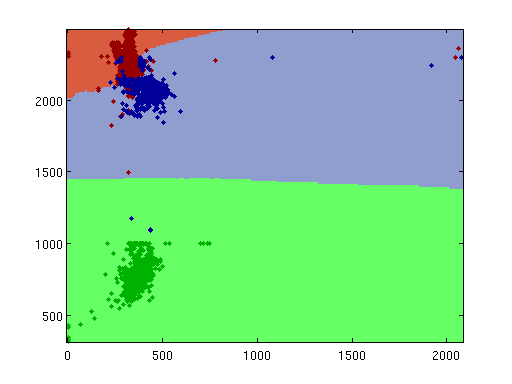
\includegraphics[clip, trim=40px 15px 30px 10px]{knn_real.png}
\caption{KNN, $K=40$}
\end{figure}

\begin{figure}[htbp!]
\center
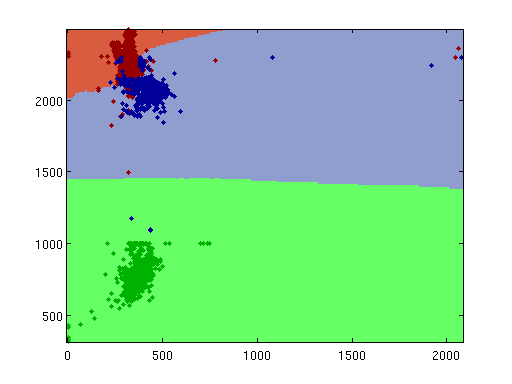
\includegraphics[clip, trim=40px 15px 30px 10px]{knn_real.png}
\caption{KNN, $K=60$}
\end{figure}


\end{document}

